\documentclass[12pt]{article}

%
%Margin - 1 inch on all sides
%
\usepackage[letterpaper]{geometry}
\usepackage{times}
\geometry{top=1.0in, bottom=1.0in, left=1.0in, right=1.0in}

%
%Doublespacing
%
\usepackage{setspace}
\doublespacing

%
%Rotating tables (e.g. sideways when too long)
%
\usepackage{rotating}

%
%Hyperlinks
%
\usepackage{hyperref}
\hypersetup{
    colorlinks=true,
    linkcolor=black,
    filecolor=magenta,      
    urlcolor=black,
    pdftitle={AP Statistics Project},
    pdfpagemode=FullScreen,
    }

%
%Inline code blocks
%
\usepackage{minted}
\usemintedstyle{vs}

%
%Table
%
\usepackage{booktabs, multirow} % for borders and merged ranges
\usepackage{soul} % for underlines
\usepackage[table]{xcolor} % for cell colors
\usepackage{changepage,threeparttable} % for wide tables

%
%Images (for graphs)
%
\usepackage{graphicx}
\graphicspath{ {./images/} }

%
%Fancy-header package to modify header/page numbering (Waugh)
%
\usepackage{fancyhdr}
\pagestyle{fancy}
\lhead{} 
\chead{} 
\rhead{Waugh \thepage} 
\lfoot{} 
\cfoot{} 
\rfoot{} 

\renewcommand{\headrulewidth}{0pt} 
\renewcommand{\footrulewidth}{0pt} 
%To make sure we actually have header 0.5in away from top edge
%12pt is one-sixth of an inch. Subtract this from 0.5in to get headsep value
\setlength\headsep{0.333in}
%To fix some error thingy with dimensions lol
\setlength{\headheight}{15pt}
\addtolength{\topmargin}{-2.5pt}

%
%Begin document
%
\begin{document}
\begin{flushleft}
	
	%%%%First page name, class, etc
	Miles Waugh\\
	Mr. Palm\\
	AP Statistics C°\\
	November 29 2022\\
	
	
	%%%%Title
	\begin{center}
		Do More Popular Scratchers Receive More Loves per View on Average?
	\end{center}
	
	
	%%%%Changes paragraph indentation to 0.5in
	\setlength{\parindent}{0.5in}
	%%%%Begin body of paper here
	
	%
	% Introduction
	%

	% Background
	Scratch is a high-level block-based visual programming language and website aimed primarily at children as an educational tool for programming, with a target audience of ages 8 to 16 (though I know several much older people who still use it for various reasons). Users on the site, called Scratch users, Scratchers, or users, can create projects on the website using a block-like interface. Publicly-posted projects may receive views, loves, and favorites from other users. Views are counted as the number of times a user runs a project for the first time after loading the project, and each user can choose to love and/or favorite a project once. Users can also follow each other, and it does not have to be a mutual connection.
	Scratch is very dear to my heart, because it was one of the first programming languages I ever used. I made my first account 8 years and 4 months ago, and it enabled me to express creative problem-solving outside the apparent rigid nature of elementary school. As a result, I wanted to do my AP Statistics project on data collected from the Scratch website. I hope to learn more about the relationships between different project statistics.
	
	I will be investigating the relationship between Scratcher popularity and how likely their projects are to be ‘loved’ by a viewer. I will measure the Scratcher’s popularity by the number of followers that Scratcher has, and I will measure ‘love’ likelihood as the average ratio between total loves and views on all public, published, and visible projects that the Scratcher has produced.
	
	% Hypothesis
	I predict that more popular Scratchers will receive fewer loves per view on average than less popular Scratchers, largely due to the demographics of viewers on various kinds of projects. Scratchers with minimal follow counts likely do not produce favorable projects, which their follow count reflects, and would therefore have a low love-to-view ratio. Younger Scratchers also commonly participate in a practice called ‘F4F’ (follow-for-follow), where both users agree to follow each other. The Scratchers then ‘love’ each other’s projects in order to mutually boost each others’ popularity. This would cause an increase in the love-to-view ratio in users with a decently large following. Users with a massive following usually gain their follower base through either well-made video games, or through affiliation with Scratch (e.g., by being on the Scratch Team, being a senior developer for Scratch Addons, etc.). Blindly following members of the Scratch Team despite their lack of quality projects on the platform, or avoiding internet filters for online gaming websites by playing Scratch remakes, tends to attract the same crowd of users: the extremely little kids who do not know or want to learn to code, and who likely do not tend to love and favorite projects since they have a less genuine appreciation for them. I would expect this to reduce the love-to-view ratio in Scratchers with massive follow bases, hence making the overall association negative.
	
	% Method	
	To extract and collect data from the Scratch website, I used the \hyperlink{https://api.scratch.mit.edu/}{Scratch API}. My code is posted publicly \hyperlink{https://github.com/piano-miles/Scratch-Userdata}{on GitHub}, and the data can be collected by running \mintinline{sh}{./local/main.py} with Python 3. I suggest leaving at least 4 GB of RAM available for running the full data collection process.
	
	%
	% Graphs
	%

	% Original scatterplot
	\newpage
	\begin{figure}[h]
		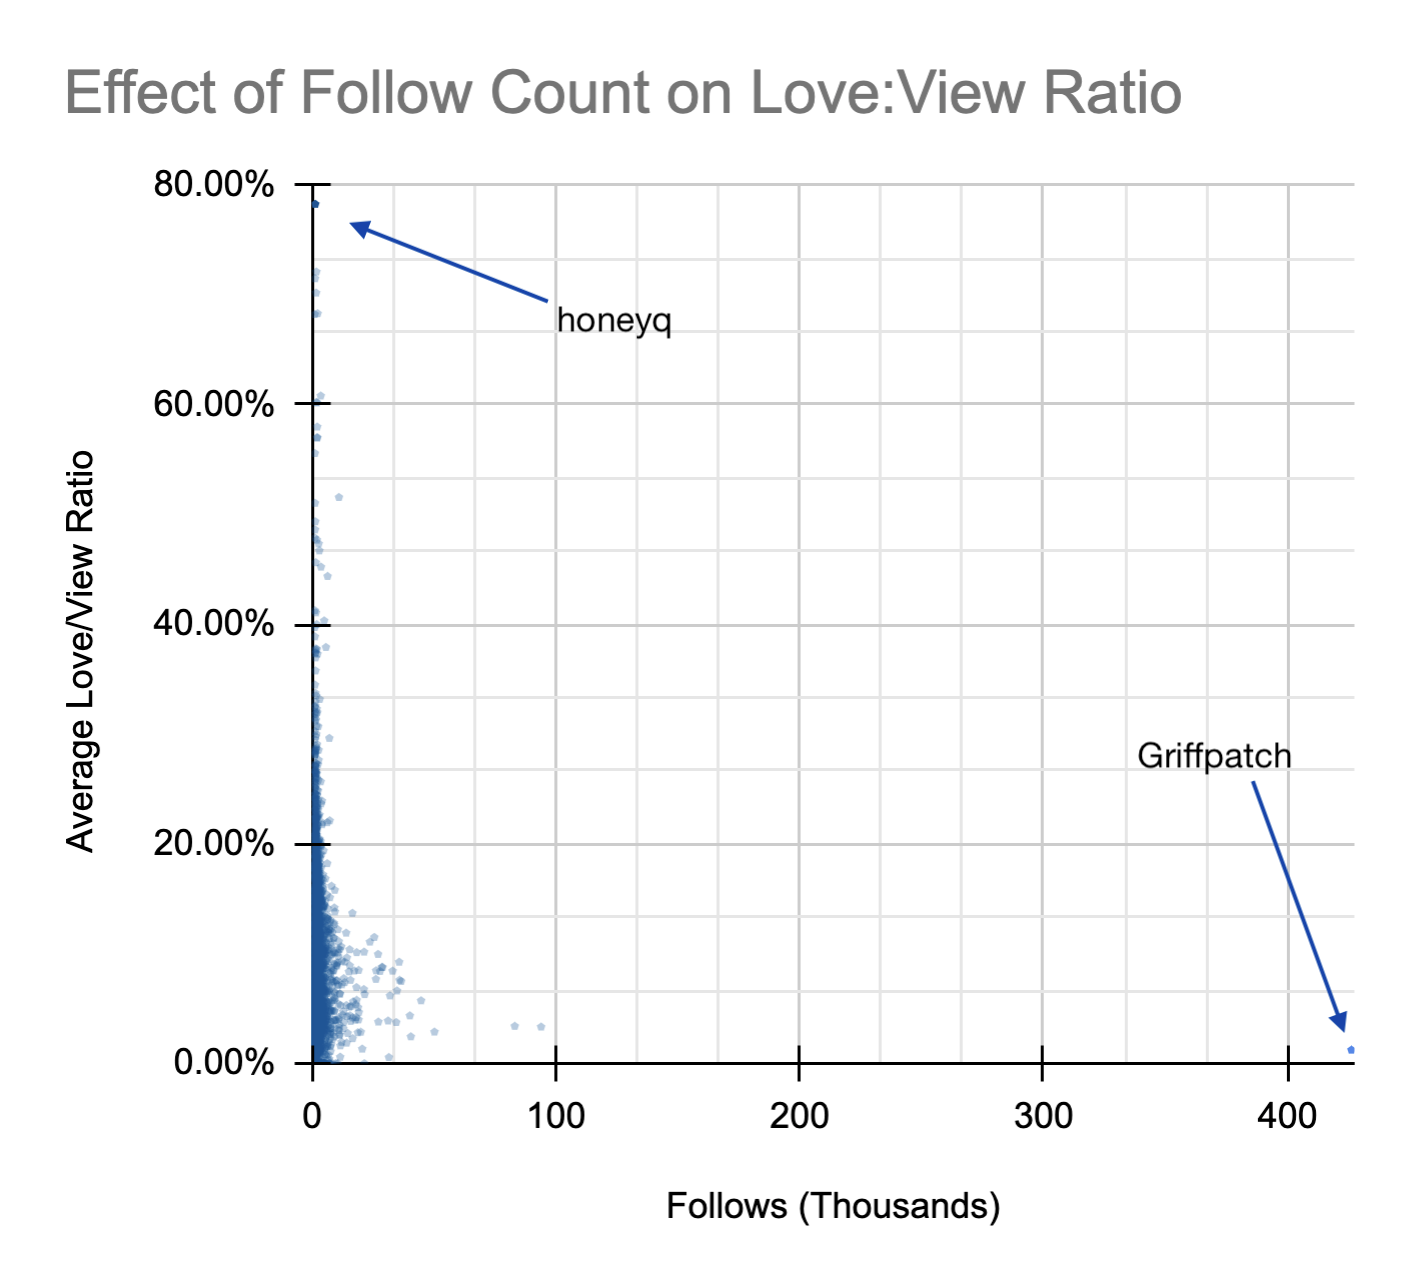
\includegraphics[width=\linewidth]{img/plot1.png}
		\centering
	\end{figure}
	
	% Re-expressed scatterplot
	\newpage
	\begin{figure}[h]
		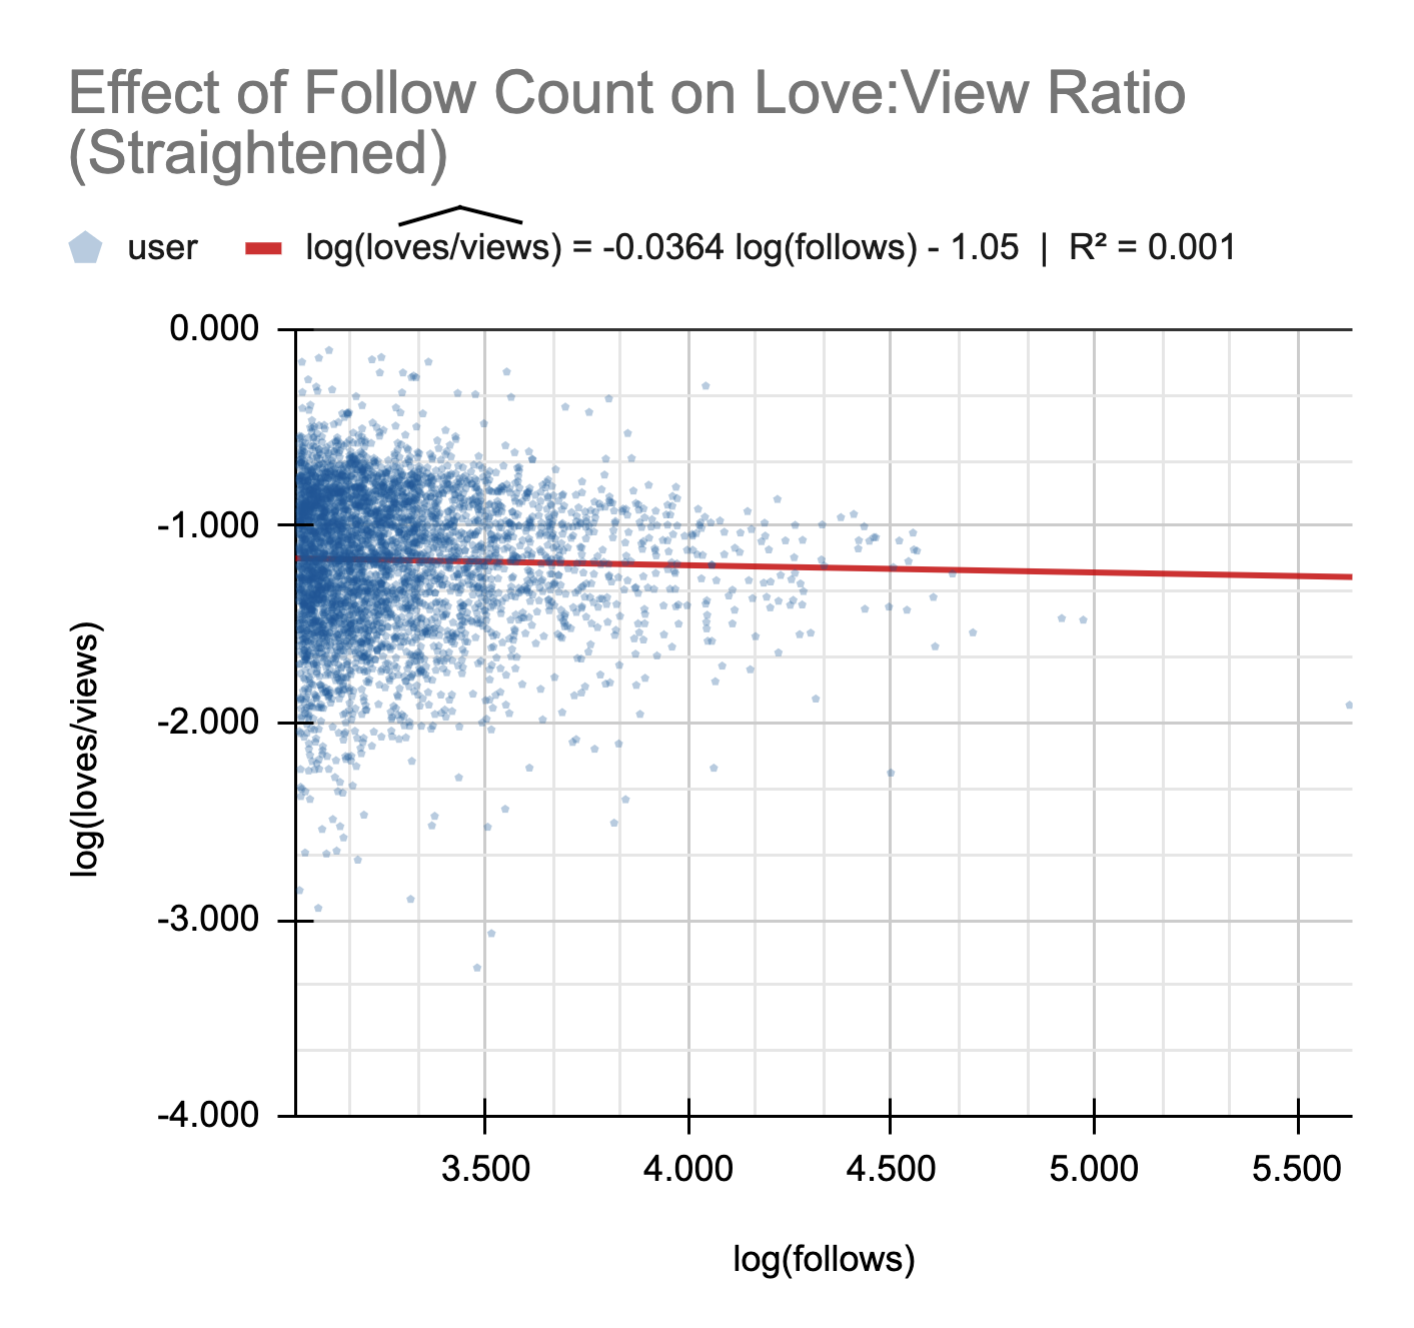
\includegraphics[width=\linewidth]{img/plot2.png}
		\centering
	\end{figure}
	
	% Residual plot
	\newpage
	\begin{figure}[h]
		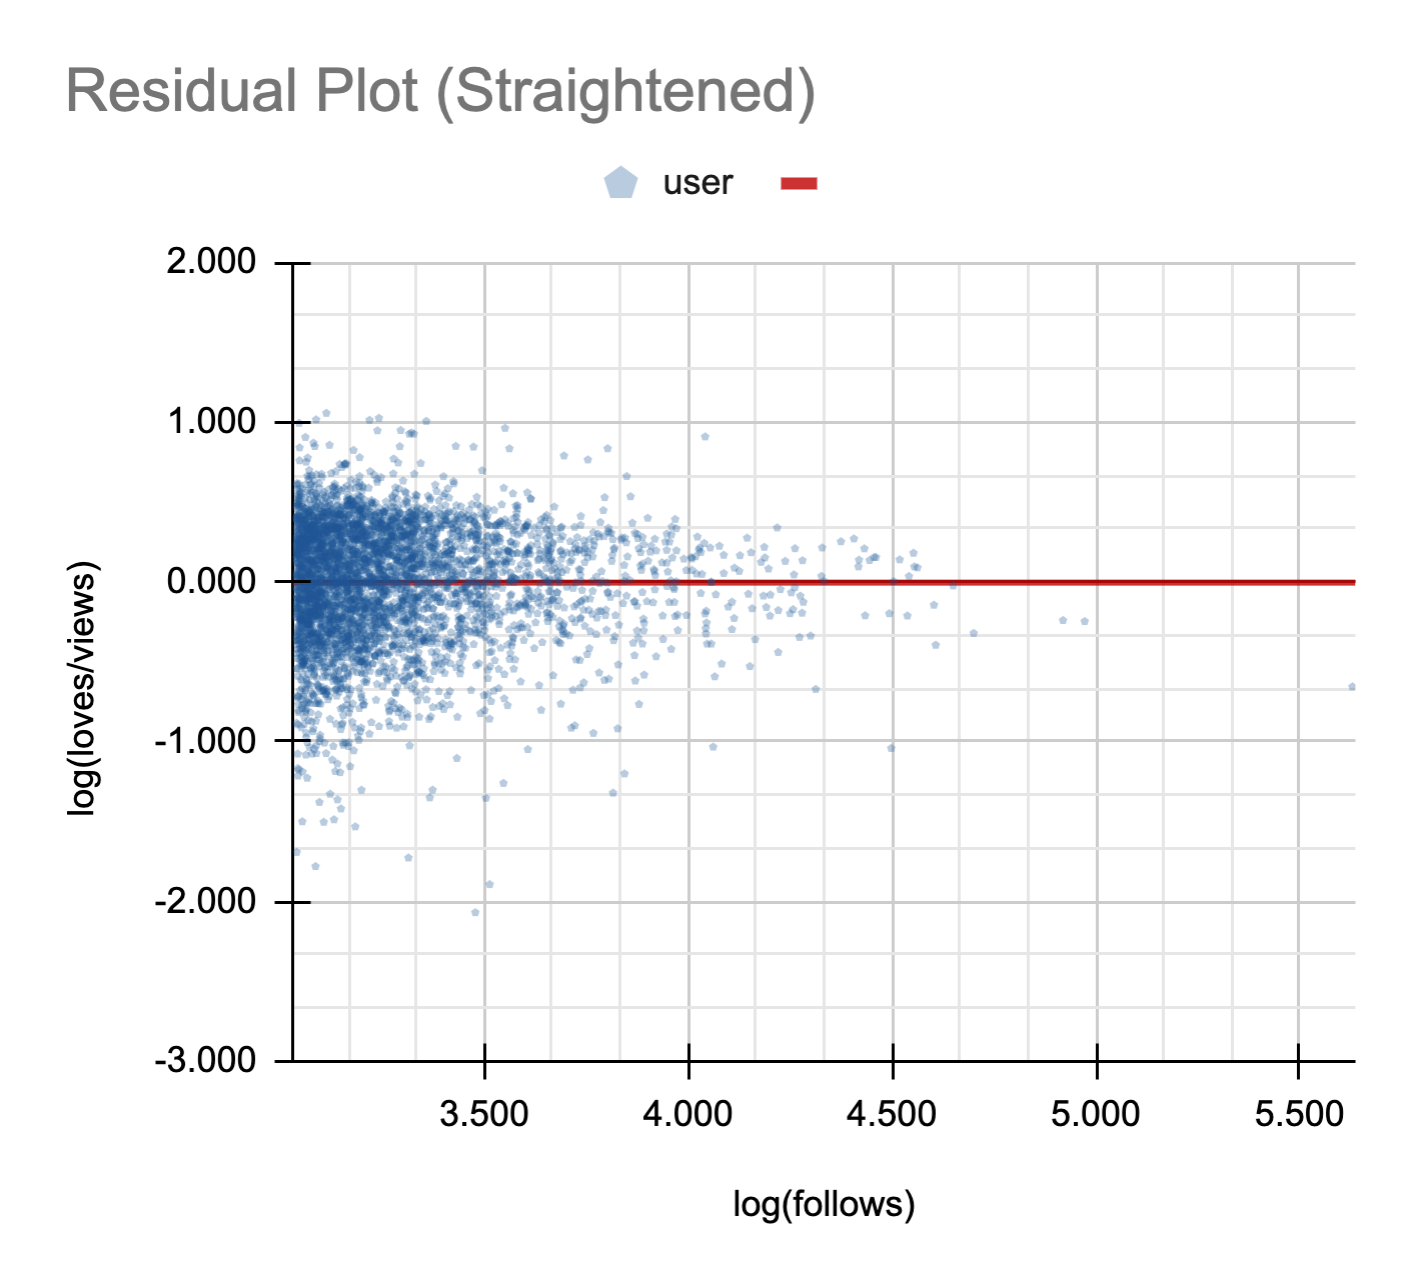
\includegraphics[width=\linewidth]{img/plot3.png}
		\centering
	\end{figure}
	
	% Analysis
	The data in the original scatter plot is highly concentrated in the bottom-left corner of the graph (a right skew in the distribution for loves/views and an even heavier right skew in the distribution for follows). I, therefore, chose to re-express the data by taking the log of both distributions in an attempt to make the distributions more uniform. The equation of the regression line is log(predicted loves/views) = –0.0364 log(follows) – 1.05. The slope is -0.0364, meaning that the love/view ratio will tend to decrease by $1-10^{-0.0364}=$ 8.03978…\% for a 10-fold increase in follower count, according to the model. The y-intercept is -1.05, meaning the love-to-view ratio is approximately $10^{-1.05}=$ 8.9125…\% when the follower count is 1, according to the model.
	
	The $R^2$ value is extremely low, at just 0.001. That means that only about 0.1\% of the variation in log(loves/views) can be attributed to log(follows) in the model. The residual plot is also not uniformly distributed, so there may be some other more complex association between the parameters.
	
	% Conclusion
	In conclusion, there is little association between a Scratcher’s popularity (measured by follower count) and the ratio between the number of loves and views they receive. The $R^2$ value of 0.1\% means that only about 0.1\% of the variation in log(loves/views) is accounted for by the model, which is statistically insignificant. There also appears to be little association between the two parameters, visually.
	
\end{flushleft}
\end{document}
\}